\section{What Pathways are Important?}

% \subsection{Damage Repair}

% \begin{frame}[c]{DNA Damage Response}
%     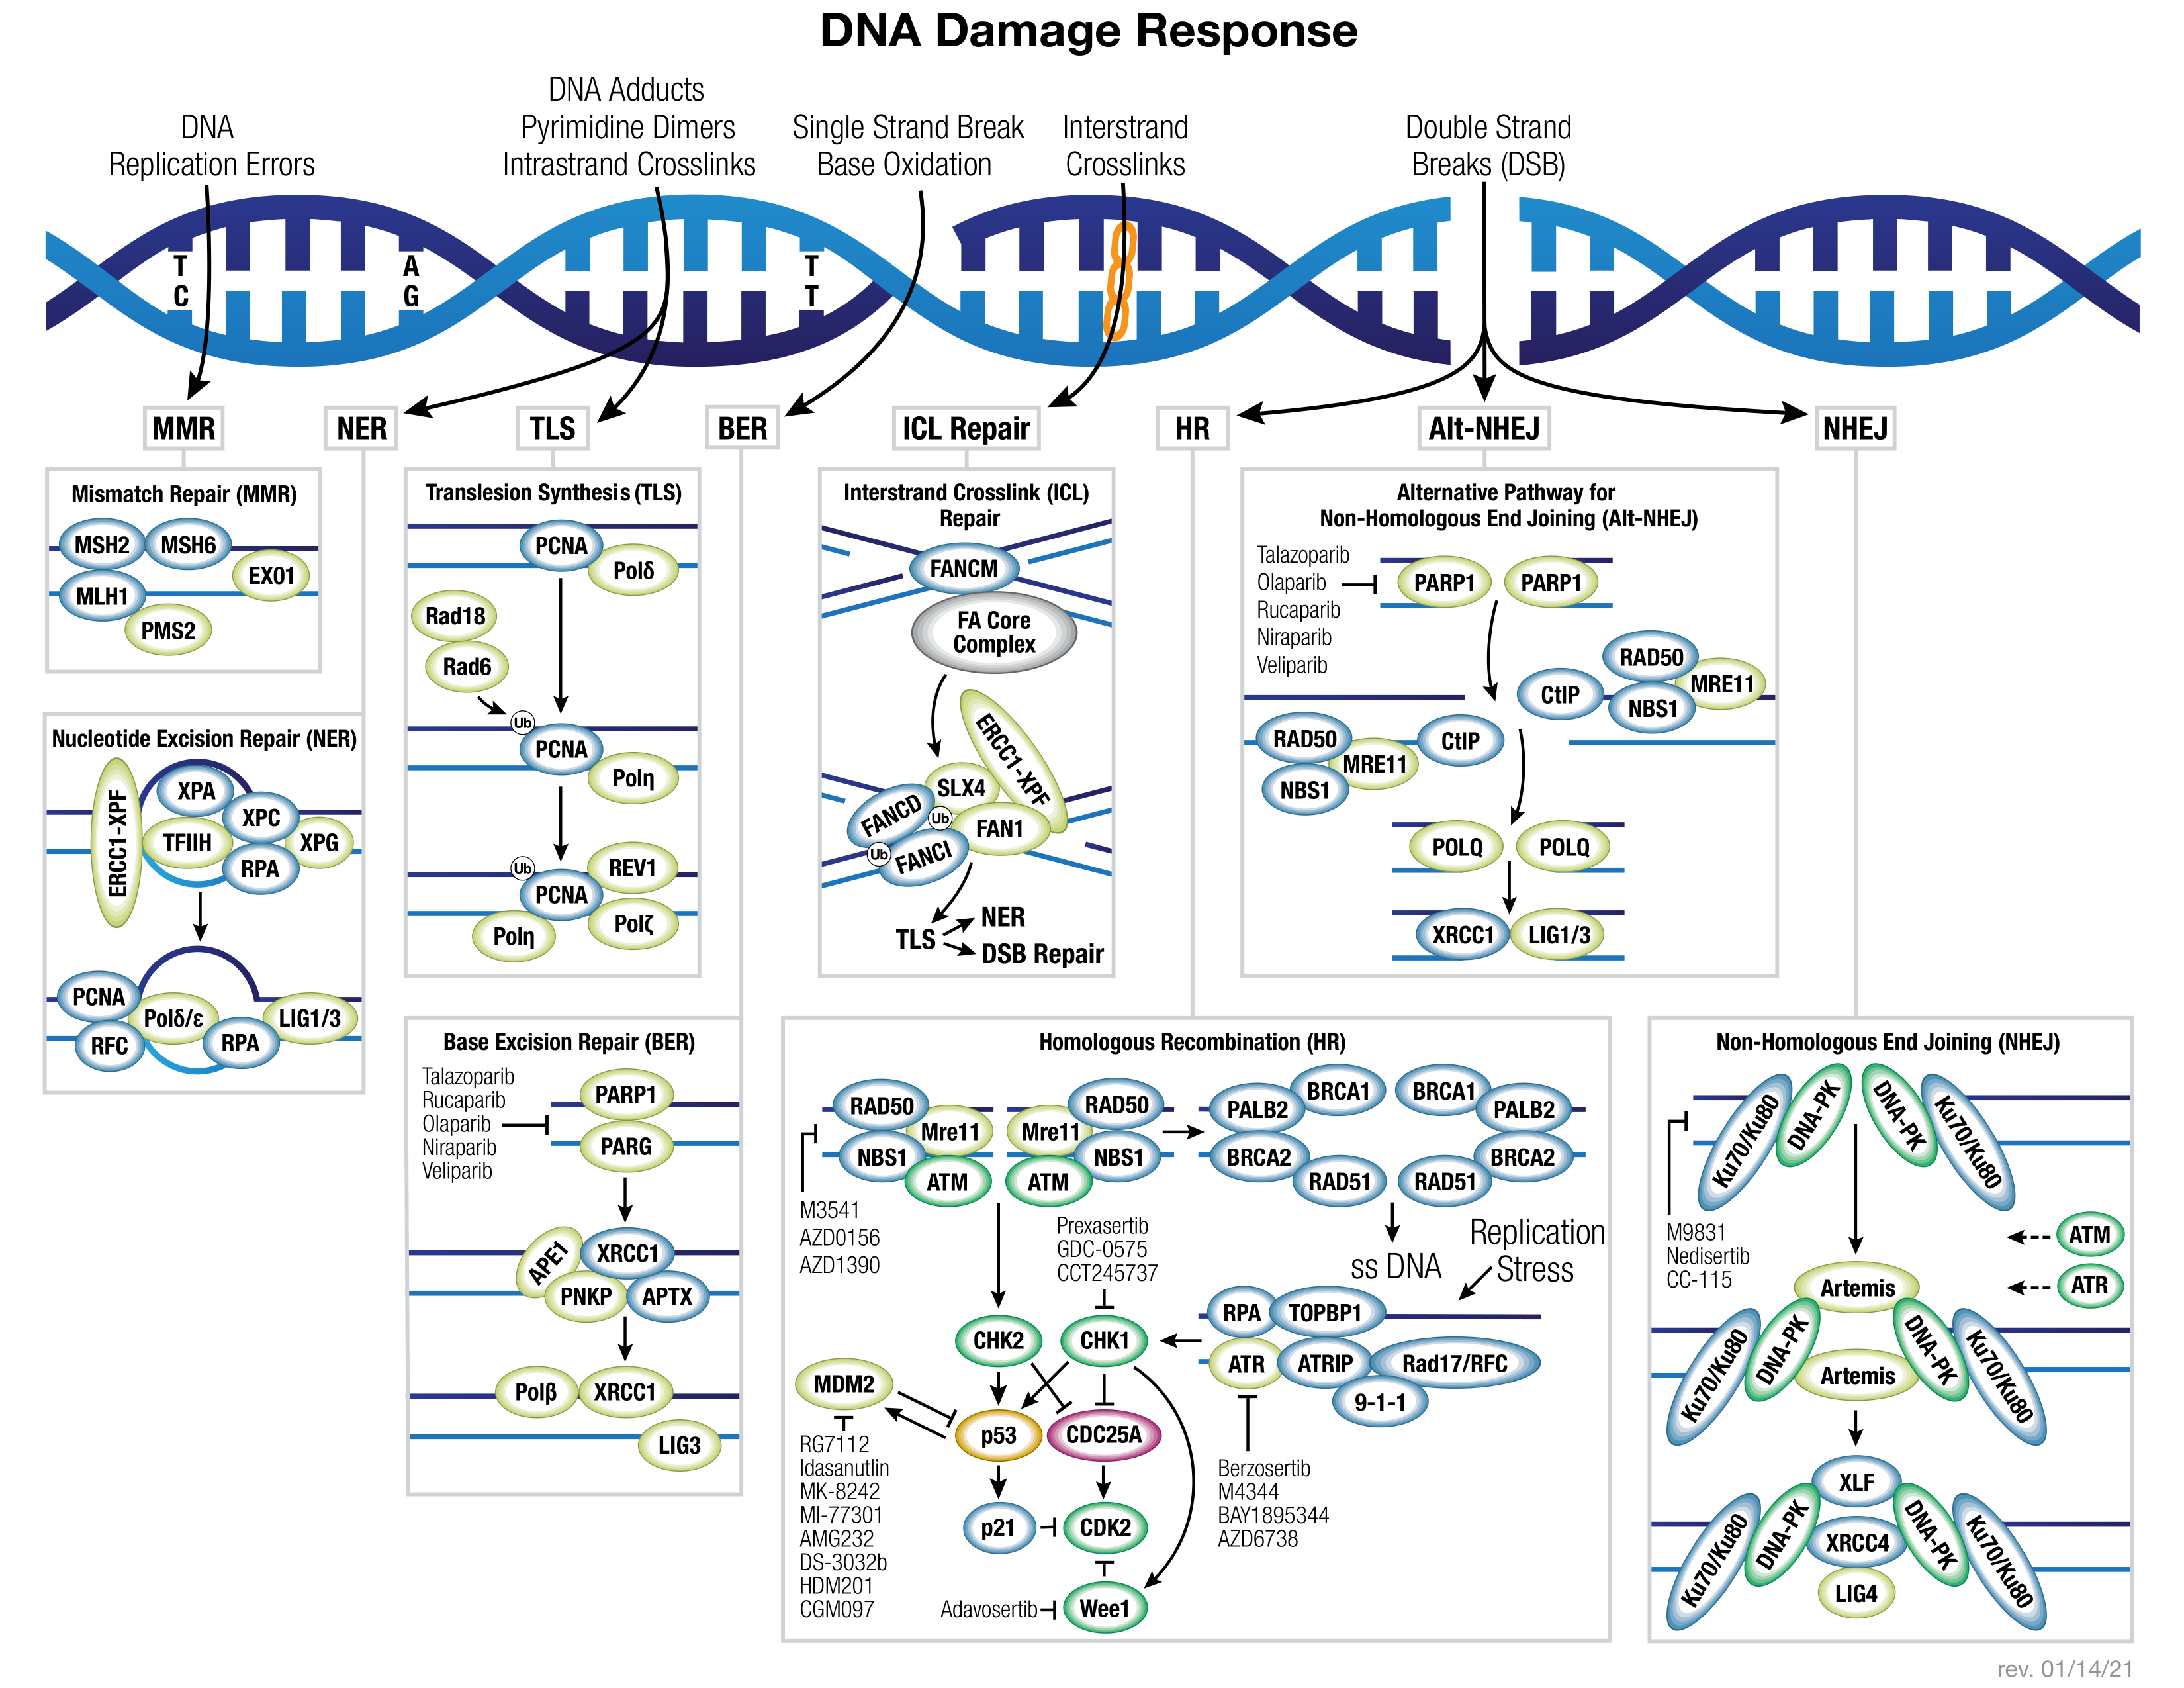
\includegraphics[height=0.85\textheight]{DNA-Damage-Response_2} \\
%     Source: \cite{DNADamag68:online}
%     \pnote{Not sure what I want to say here?}
% \end{frame}


\subsection{Dietary Restriction}

% \begin{frame}[c]{Calorie Restriction Pathways}
%     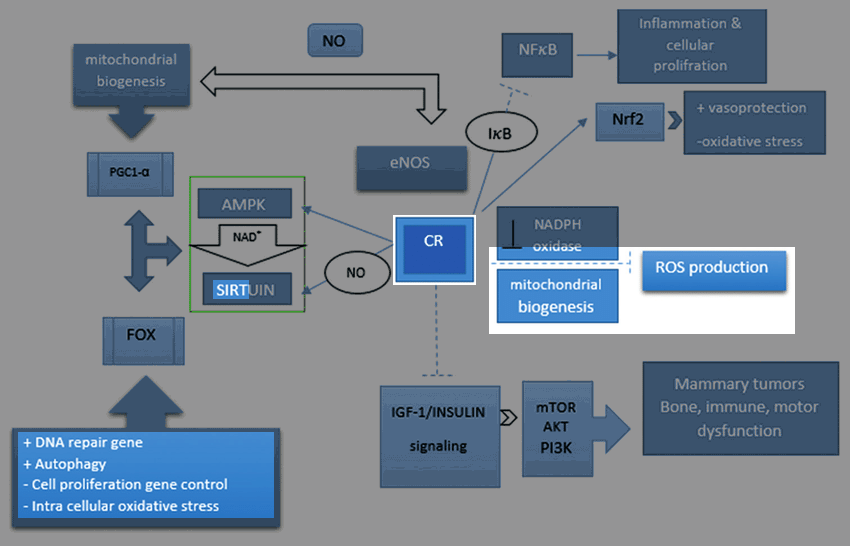
\includegraphics[height=0.85\textheight]{cr_pathways_highlights} \\
%     Source: \cite{hanjani2018protein}, highlights added
% \end{frame}
\subsection{Senescence Feedback Loops}


\begin{frame}[c]{Inflammation Effects}
    \begin{aquote}{\cite{NintilTh68:online}}
        {\em Also, the environment that inflammation creates is one that is} meant to
        increase cell turnover {\em (More apoptosis, but also more cell growth to
        replace lost cells), with granulocytes secreting toxic agents
        (Including ROS) to make the area affected less hospitable (But also
        increases damage to DNA), and specific cytokines like the} tumor
        necrosis factor that induce cell death, and growth factors that promote
        cell growth.
    \end{aquote}
\end{frame}

\begin{frame}[c]{Senescent Cell Effects}
    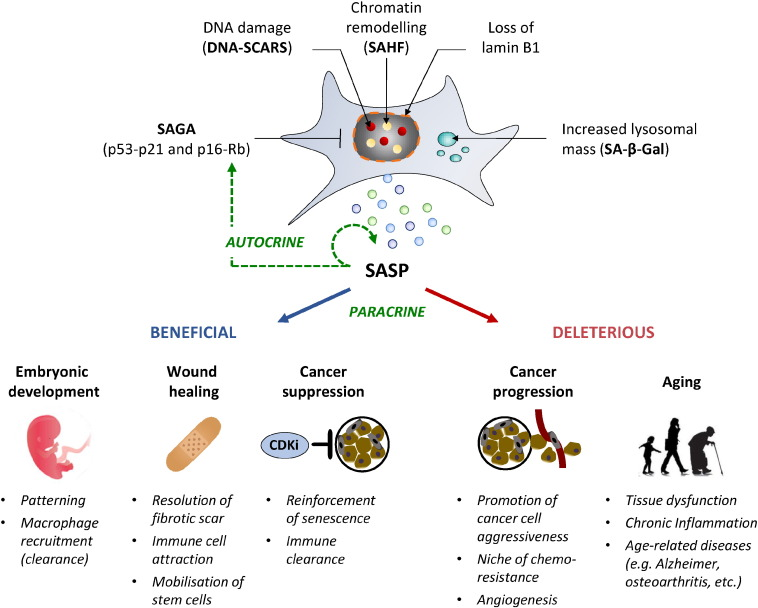
\includegraphics[height=0.85\textheight]{sasp_effects} \\
    Source: \cite{malaquin2016keeping}
\end{frame}

% \begin{frame}[c]
%     Feedback loop 1: mitochondrial high ROS-state (due to emergency state) and resulting DNA-damage causing prolonged emergency state
%     Feedback loop 2: repair pathways fixing dna damage unrestraining transposons proliferating and causing further dna damage
%     resulting in SASP
% \end{frame}
